
%Volume: maximaal aantal pagina van inleiding t/m literatuur, maximaal  35 bladzijden (excl.bijlagen).
\documentclass[11pt]{report}
\usepackage[a4 paper, headheight=1pt, headsep=1pt] {geometry}
\usepackage{titlesec}
\titleformat{\chapter}[display]   
{\normalfont\huge\bfseries}{\chaptertitlename\ \thechapter}{8pt}{\huge}   
\titlespacing*{\chapter}{0pt}{-65pt}{8pt}
\titlespacing*{\section}{0pt}{5pt}{1pt}
\setlength{\parindent}{0pt}
\setlength{\parskip}{5pt plus 2pt minus 1pt}
\setlength{\textheight}{680pt}
\setlength{\headsep}{0pt}
%\usepackage{showframe}
\usepackage{graphicx}
\usepackage[usenames,dvipsnames]{color}
%\usepackage{picins}
\footskip = 20pt 
\usepackage[nodayofweek]{datetime}
\usepackage{tikz}
\usepackage{todonotes}


\usepackage{pdfpages}
\usepackage{siunitx}
\usepackage[HTML]{xcolor}
\usepackage{multirow,colortbl,array}


\begin{document}
\begin{titlepage}
	\begin{center}
	\vspace*{0\textheight}\todo{again UU?}
	{\scshape\LARGE Utrecht University \par} 
	\vspace{1cm} 
	\line(4,0){300}
	\vspace{0.5cm} \\
	{\Large \bfseries Local characteristics of two Svalbard glaciers\\}
	\vspace{0.5cm}
	\line(4,0){300} \\

	\vspace{2.5cm}
	\begin{minipage}[t]{0.4\textwidth}
	\begin{flushleft} \large
	\emph{Authors:}\\
	{Isolde Glissenaar}\\
	{Daphne van Zanten} \\
	\end{flushleft}
	\end{minipage} %No ENTER BECAUSE!
	\begin{minipage}[t]{0.4\textwidth}
	\begin{flushright} \large
	\emph{Supervisor:} \\
	{Dr. C.H. Tijm-Reijmer}\\
	\end{flushright}
	\end{minipage}\\[0.4cm]

	\vspace{3.5cm} \todo{picture?}
	\large \textit{}\\[1cm]

	{\large {\today}\\[2cm] % Date

	\noindent
	
\includegraphics[scale=1, width=0.4\textwidth]{UU-logo.jpg}
	\hspace{0.2\textwidth}
	
\includegraphics[scale=1, width=0.22\textwidth]{imau.png}}
	\end{center}
\end{titlepage}

\newpage
\tableofcontents

\chapter{Introduction}\label{sec:intro}
\pagenumbering{arabic}
\setcounter{page}{2}
%\todo{In report: \\
%- General description experiment and conditions\\
%– General description of the dataset and data handling\\
%– Detailed analyses of chosen subject\\
%+- 15 pages}

Around 1595, a Dutch man called Willem Barentsz went on expedition to search for a North East Passage when he discovered Svalbard \cite{sval}. To imagine this situation, a painting of his ship is made by Arnold de Lange and shown in Figure \ref{fig:wbs}. From this moment on, Dutch people invested in research on Svalbard's climate and ecology. Around 2010, the interest in research on the eastern side of the island Spitsbergen increased. However, there is a small amount of data from this part of the archipelago. To investigate the present situation and organize a new expedition to this part of the archipelago, SEES (Netherlands Scientific Expedition Edge\o ya Spitsbergen) has been established, which is still active nowadays \cite{sees}. SEES organized an expedition in august 2015 during which an Automatic Weather Station was installed on the Ulvebreen.

\begin{figure}[h]
\includegraphics[scale=1, width=0.5\textwidth]{wbs.jpg}
\centering{}
\caption{Ship of Willem Barentsz at the discovery of Svalbard, made by Maritim painter Arnold de Lange}
\label{fig:wbs}
\end{figure}

In our project, we retrieved measurement data from three weather stations in Svalbard. Two are located on glaciers (Nordenski\H{o}ldbreen and Ulvebreen) and one on land (Svalbard Lufthavn). In this study, measurement data from the three locations on Svalbard is used to answer the following question:

\textit{How can the local characteristics of two Svalbard glaciers be explained?}

To investigate this, sub-questions arise:
\textit{What are the characteristics of the Nordenski\H{o}ldbreen and the Ulvebreen?} and \textit{What are the differences between the two glaciers?}

Explained in chapter \ref{sec:method} is the origin of the measurements and the data handling methods. Chapter \ref{sec:results} contains results of this research, obtained by comparing data. In chapter \ref{sec:discussion} results are discussed and compared with the hypothesis. In chapter \ref{sec:conclusion}, a conclusion is presented.

\newpage

\chapter{Method}\label{sec:method}

To investigate the local characteristics of two glaciers on Svalbard, the location of the glaciers are described in section \ref{sec:loc}. On those glaciers, instruments are installed to measure different variables, which are described in section \ref{sec:instr}. Finally, the data handling is discussed in section \ref{sec:datah}.

%\textcolor{red}{location of measurements, instruments, data handling (on making the daily averages and handling the data gaps.)} are investigated. 

\section{Location} \label{sec:loc}
\todo{bronnen}
This study discusses data from weather stations situated on Svalbard, which is a Norwegian archipelago in the Arctic Ocean, north of the European mainland. The island group ranges from 74$^\circ$N to 81$^\circ$N in latitude. The archipelago features an Arctic climate, although with higher temperatures than other areas on the same latitude.  The northernmost branch of the relatively warm North Atlantic Current, the West Spitsbergen Current (Figure \ref{fig:current}), moderates the temperature on the western side of the island. The East Spitsbergen Current brings colder water from higher latitudes to the eastern side of the archipelago. The mean temperatures range from $\SI{-16}{^\circ C}$ in February to $\SI{6}{^\circ C}$ in July (Norwegian Meteorological Institute) at Svalbard Lufthavn, in the middle of the main island Spitsbergen. The mean yearly precipitation at Svalbard Lufthavn is 190 mm. 
 

\begin{figure}[h]
\includegraphics[scale=1, width=0.5\textwidth]{currents_svalbard.jpg}
\centering{}
\caption{Map of Svalbard showing key features and major ocean currents (Storrie et al., 2018).}
\label{fig:current}
\end{figure}

All three measurement locations are situated on the largest island, called Spitsbergen. Data is used from two weather stations from the Institute for Marine and Atmospheric research Utrecht (IMAU) located on two glaciers, and data from an operational station from the Norwegian Meteorological Institute (Figure \ref{fig:locations}).

\begin{figure}[h]
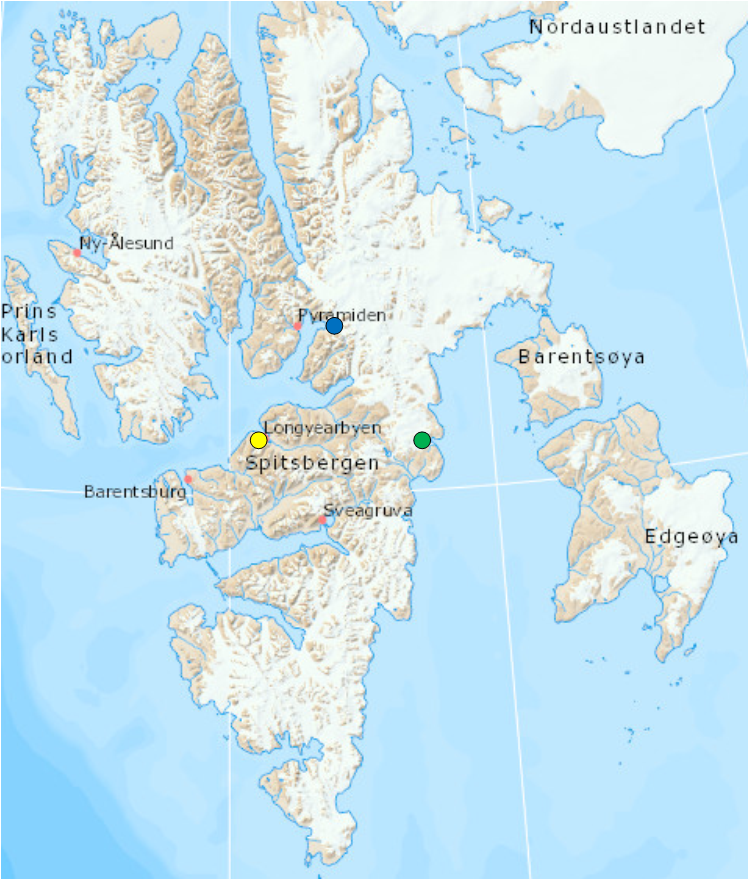
\includegraphics[scale=1, width=0.5\textwidth]{svalbard_locations.png}
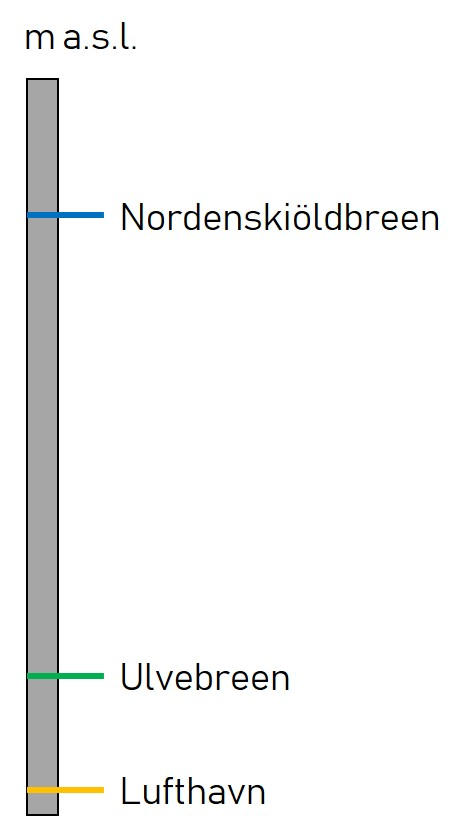
\includegraphics[scale=1, width=0.33\textwidth]{height.jpg}
\centering{}
\caption{Left: Map (Norwegian Polar Institute) of Svalbard showing the locations of the weather stations. Blue: Nordenski\H{o}ldbreen, green: Ulvebreen, yellow: Svalbard Lufthavn. Right: Schematic picture of differences in height}
\label{fig:locations}
\end{figure}

The weather stations are situated on the Nordenski\H{o}ldbreen and the Ulvebreen. The Nordenski\H{o}ldbreen is a marine-terminating glacier, terminating in Adolfsbukta, which is a branch of Billefjorden. The glacier is situated roughly in the middle of the island Spitsbergen. The glacier is $\SI{25}{km}$ long, $\SI{11}{km}$ wide and located 529 meters above sea level (m a.s.l.). It originates from Lomonosovfonna and flows in southwesterly direction (Figure \ref{fig:norden}). 

The Ulvebreen is also a marine-terminating glacier. This glacier is a tributary to Nordmannsfonna and terminates in Dunérbukta, at the east of Spitsbergen. The Ulvebreen is $\SI{9}{km}$ long, $\SI{2.5}{km}$ wide and located at 140 m a.s.l., which is a difference of 389 meter compared to the Nordenski\H{o}ldbreen. It flows in southeasterly direction (Figure \ref{fig:ulve}). 

The third measurement location is an operational station at Svalbard Lufthavn, close to the largest settlement on Svalbard: Longyearbyen. This operational station is run by the Norwegian Meteorological Institute. Svalbard Lufthavn is located at Adventfjorden, which debouches into Isfjorden. It has a height of 28 m a.s.l., which is a difference of 501 meter with the Nordenski\H{o}ldbreen and 112 meter with the Ulvebreen, also schematically drawn in Figure \ref{fig:locations}.

\begin{figure}[h]
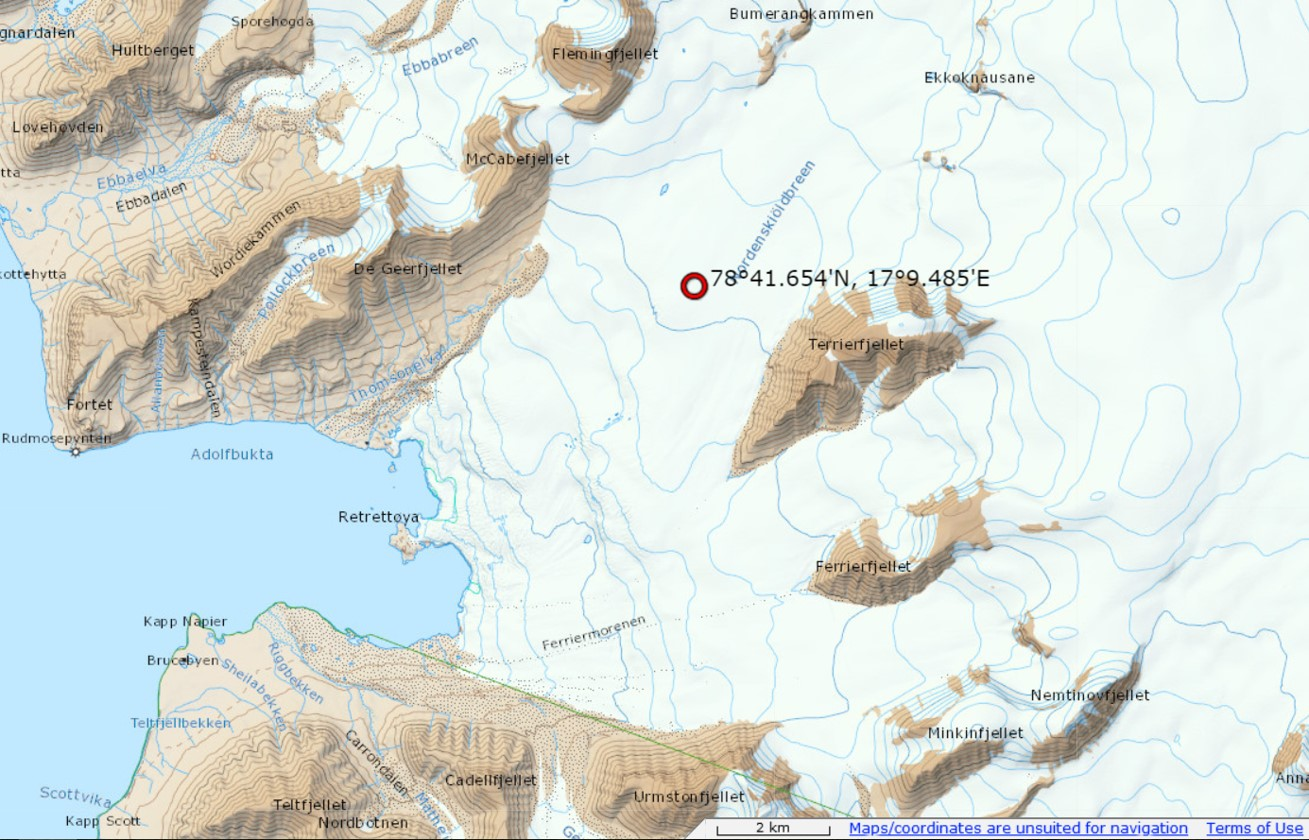
\includegraphics[scale=1, width=0.45\textwidth]{nskimap.jpg}
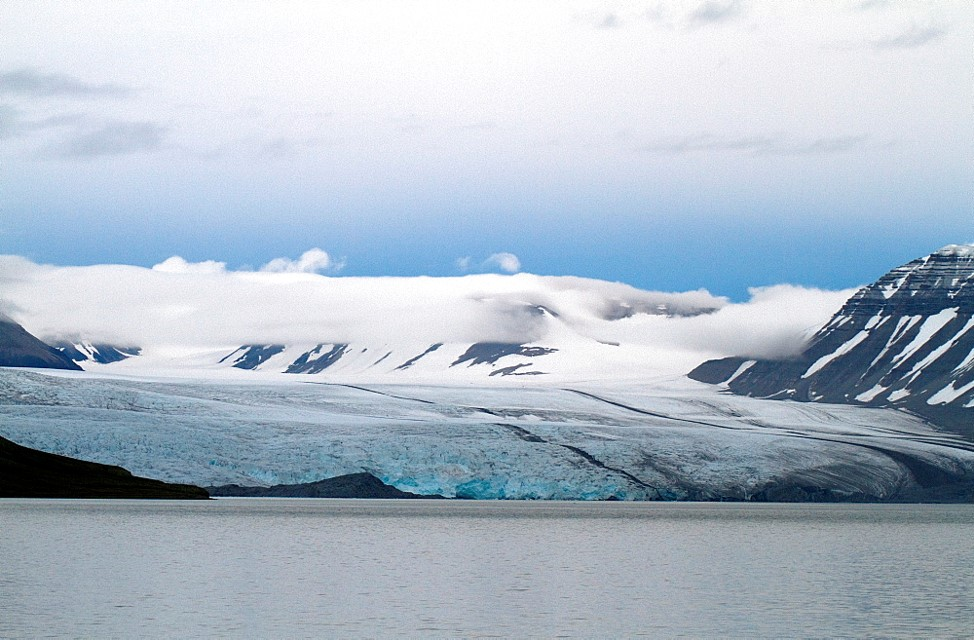
\includegraphics[scale=1, width=0.45\textwidth]{view1.jpg}
\centering{}
\caption{Left: Map showing the Nordenski\H{o}ldbreen and the location of the weather station (toposvalbard). Right: A picture of the terminus of the Nordenski\H{o}ldbreen in Adolfsbukta.}
\label{fig:norden}
\end{figure}

\begin{figure}[h]
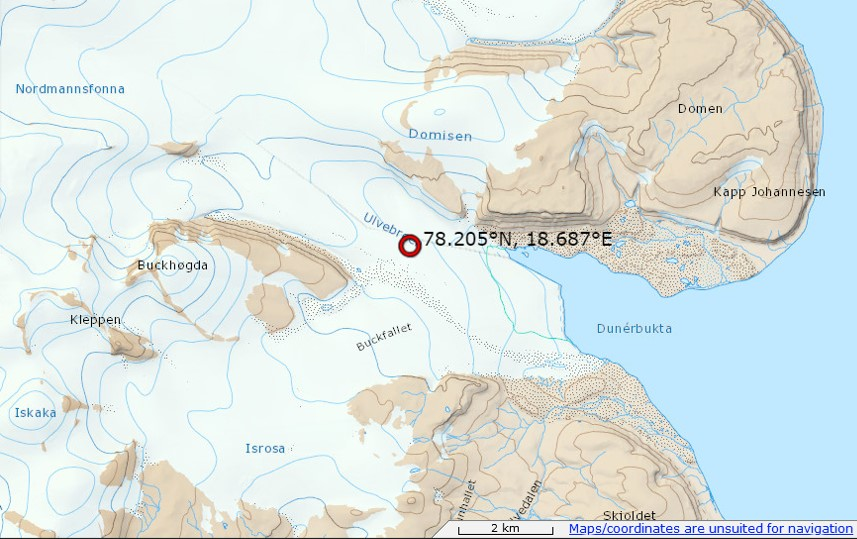
\includegraphics[scale=1, width=0.45\textwidth]{ulvemap.jpg}
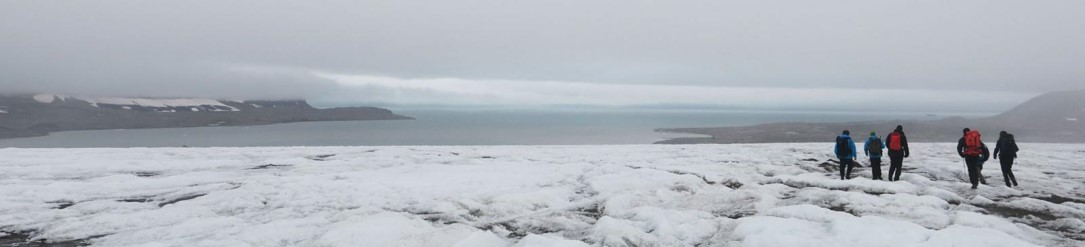
\includegraphics[scale=1, width=0.45\textwidth]{view2.jpg}
\centering{}
\caption{Left: Map showing the Ulvebreen and the location of the weather station (toposvalbard). Right: A picture made on top of the Ulvebreen (IMAU).}
\label{fig:ulve}
\end{figure}

\newpage
\section{Instruments}\label{sec:instr}
\todo{figures met kleine letters} 
Measurement data used for this study is mainly retrieved from two Automatic Weather Stations (AWS) on glaciers. The AWS on the Nordenski\H{o}ldbreen is depicted in figure \ref{fig:instrn} and the AWS on the Ulvebreen in figure \ref{fig:instru}.

\begin{figure}[h]
\raggedright
\begin{minipage}{0.5\textwidth}
\centering{}
    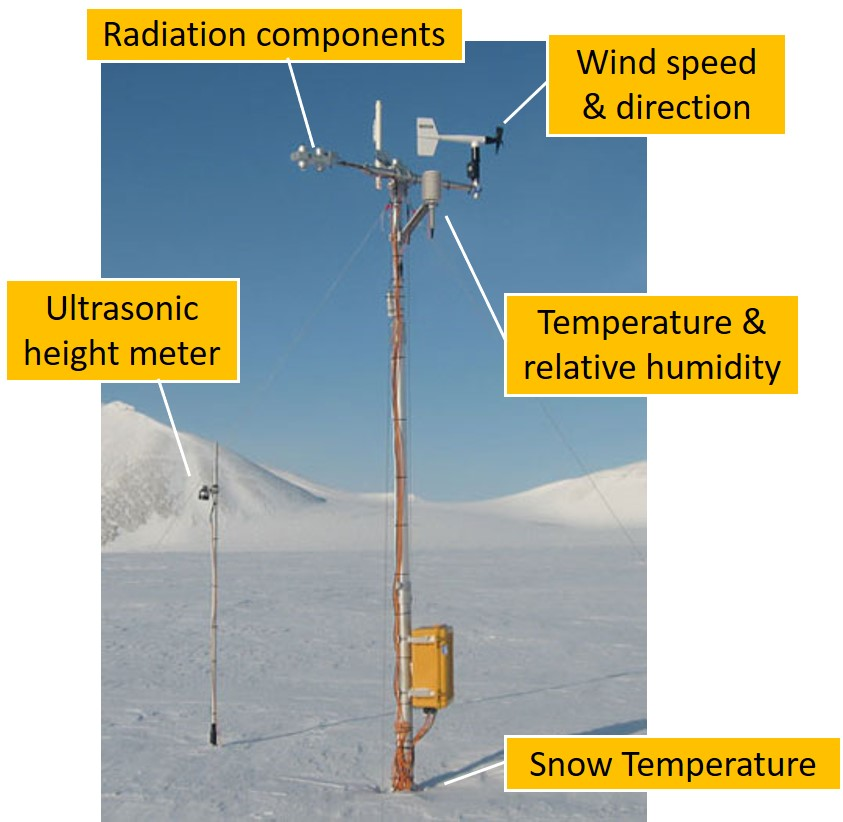
\includegraphics[width=0.9\textwidth]{nski1.jpg}
    \caption{AWS Nordenski\H{o}ldbreen \cite{uuproj}}
    \label{fig:instrn}
\end{minipage}%
\begin{minipage}{0.5\textwidth}
\centering{}
    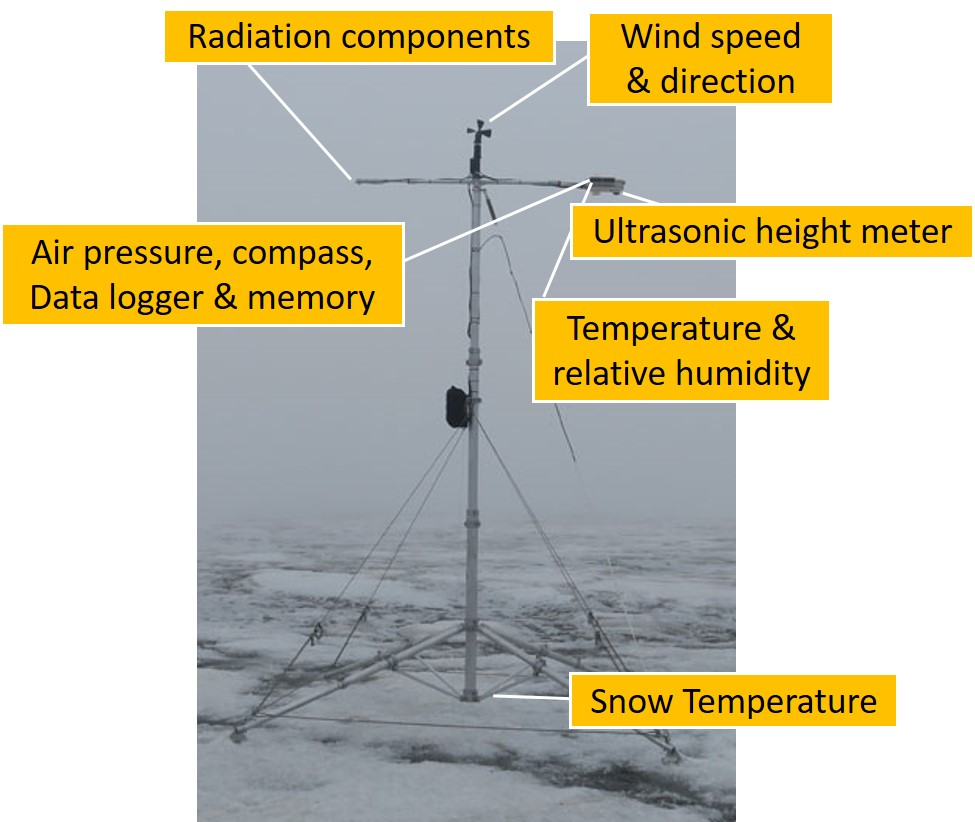
\includegraphics[width=1.05\textwidth]{ulve1.jpg}
    \caption{AWS Ulvebreen \cite{uuproj}}
    \label{fig:instru}
\end{minipage}%
\end{figure}

In figures \ref{fig:instrn} and \ref{fig:instru}, different instruments are visible, where each instrument has his own purpose. Next the different measured variables at the Nordenski\H{o}ldbreen and the Ulvebreen are explained. Finally, the used measurement data of the Lufthavn is described.\\

The AWS on the Nordenski\H{o}ldbreen was operational from March 2009 until December 2016. Within this time, measurements of different variables for timesteps of 30 minutes were saved onto the logger. Unfortunately, because of broken instruments and a location which is hard to reach, there are gaps in the measurement data for the Nordenski\H{o}ldbreen. It should be noted that the AWS on the Nordenski\H{o}ldbreen is drilled into the ice of the glacier, so the height does not change due to the melting of the ice. The weather station uses different instruments. Firstly, the temperature is measured with a thermometer. An anemometer is used to measure the horizontal wind speed and direction. A radiometer with two pyranometers is used to measure the shortwave and longwave radiation for incoming and outgoing directions. A barometer measures the pressure. The snow temperature is measured at 10 different depths. The snow height is measured with an ultrasonic sound meter. An inclinometer is used to measure the tilt.  Finally, the battery is logged as well as the temperature in the logger, to look at the status of the instruments themselves. With all those measurements, the surface temperature is derived from the outgoing longwave radiation. The potential temperature is based on the main hut temperature and pressure. The temperature at 2 meter is based on the main hut temperature and the sonic snow height. The specific humidity is based on the main hut temperature and pressure. \\

The AWS on the Ulvebreen is placed as part of the Netherlands Scientific Expedition Edge$ø$ya Spitsbergen (SEES) in August 2015 \cite{uuproj}. Like at the Nordenski\H{o}ldbreen, every 30 minutes data is saved to a logger and this process is still ongoing (the measuremnts from this station also have some data gaps). The AWS on the Ulvebreen is slightly different compared to the one on the Nordenski\H{o}ldbreen. The AWS on the Ulvebreen is positioned on top of the glacier and is therefor freely to move with the ice. This gives a different result in the snow height measurements. On the Nordenskiöldbreen (where the AWS is drilled into the ice), the snow height measurements give the height of the weather station above the top of the glacier and therefor also increases if the ice melts. On the Ulvebreen however, only the snow melt is recorded with the ultrasonic sensor. However, the AWS on the Ulvebreen also includes an ablation draw wire, which is used to study the ice melt. Figure \ref{fig:ablation} shows a schematic picture of the ablation wire. 

\begin{figure}[h]
\raggedright
\begin{minipage}{0.65\textwidth}
\raggedright
    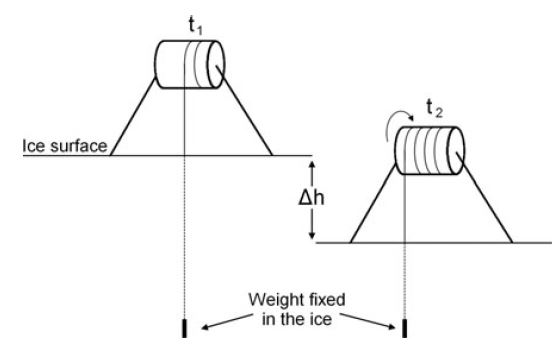
\includegraphics[scale=1, width=1\textwidth]{abliationwire.jpg}	 
    \caption{Ablation Wire \cite{abl}}
    \label{fig:ablation}
\end{minipage}%
\end{figure}

As visible in figure \ref{fig:ablation}, weights are fixed in the ice. A draw wire sensor is placed on top of the ice. This sensor is measuring the height above the fixed weight \cite{abl}. A decrease in height is caused by the ablation of the glacier.

Finally, from the observation station on Svalbard Lufthavn, only data of the wind direction and wind speed, air pressure at station level and air temperature is used to compare this with the two glaciers.

\section{Data handling}\label{sec:datah}

As described before, the dataset from the AWS on the Ulvebreen consists of data every 30 minutes from 2015-08-22 to 2018-09-13. The dataset from the Nordenski\H{o}ldbreen AWS also contains 30 minute data from 2009-03-24 to 2016-12-03. Weather data from Svalbard Lufthavn were downloaded from the Norwegian Meteorological Institute \cite{sharkii} and contains 6 hourly data from 0, 6, 12 and 18 UTC. The download consists of data from 2009-03-24 to 2018-09-13, the dates on which also data from the glaciers are available. All three datasets have a few shorter and longer gaps in measurements, caused by the failure of instruments (Ulvebreen and Nordenski\H{o}ldbreen) or too high uncertainty of the measurements (Lufthavn). To study trends in the long time series, daily averages of the data were made. The daily averages were calculated for the Ulvebreen and the Nordenski\H{o}ldbreen if at least 20 datapoints of that day were available. If there were less datapoints available the daily average was possibly not representative and thus assigned a NaN value. Because for the measurements at Lufthavn there are only measurements a day, the daily average was calculated if at least 3 datapoints were available. 

For the comparison between the three data stations, the data was cut to the period of time where all three stations have measurements, which is from 2015-08-22 to 2016-12-03. This period will from now on be called the data overlap period. Only the daily averages are used if they were calculated for all three stations. If one of them had a NaN value, this day was not used.


\newpage
\chapter{Results}\label{sec:results}
In this chapter, results of the investigation of the data are described in different sections. First, a comparison of the temperature at the weather stations is made, which is described in section \ref{sec:T}. Secondly, the wind directions differ for each glacier, which is in detail described in section \ref{sec:katw}. Finally, differences between the radiation are investigated and explained in section \ref{sec:rad}.

\section{Temperature} \label{sec:T}
\todo{alle data or gemiddelde?}
The daily average temperature at a height of two meter is compared for the Lufthavn, Ulvebreen and Nordenski\H{o}ldbreen during the data overlap period (figure \ref{fig:T2m}). From this plot, Nordenski\H{o}ldbreen seems colder than Ulvebreen, while the Lufthaven seems warmer. The mean value for the 2 meter temperature during this period is $\SI{-7.0}{^{\circ}C}$ at the Nordenski\H{o}ldbreen, $\SI{-4.9}{^{\circ}C}$ at the Ulvebreen and $\SI{-2.1}{^{\circ}C}$ at Lufthavn. The main difference between mean temperature is caused by the difference in height of the locations. The Nordenski\H{o}ldbreen is located at 529 meters a.s.l, the Ulvebreen at 140 meters a.s.l. and Svalbard Lufthavn at 28 meters a.s.l., as described in section \ref{sec:loc}. 

\begin{figure}[h]
\centering{}
    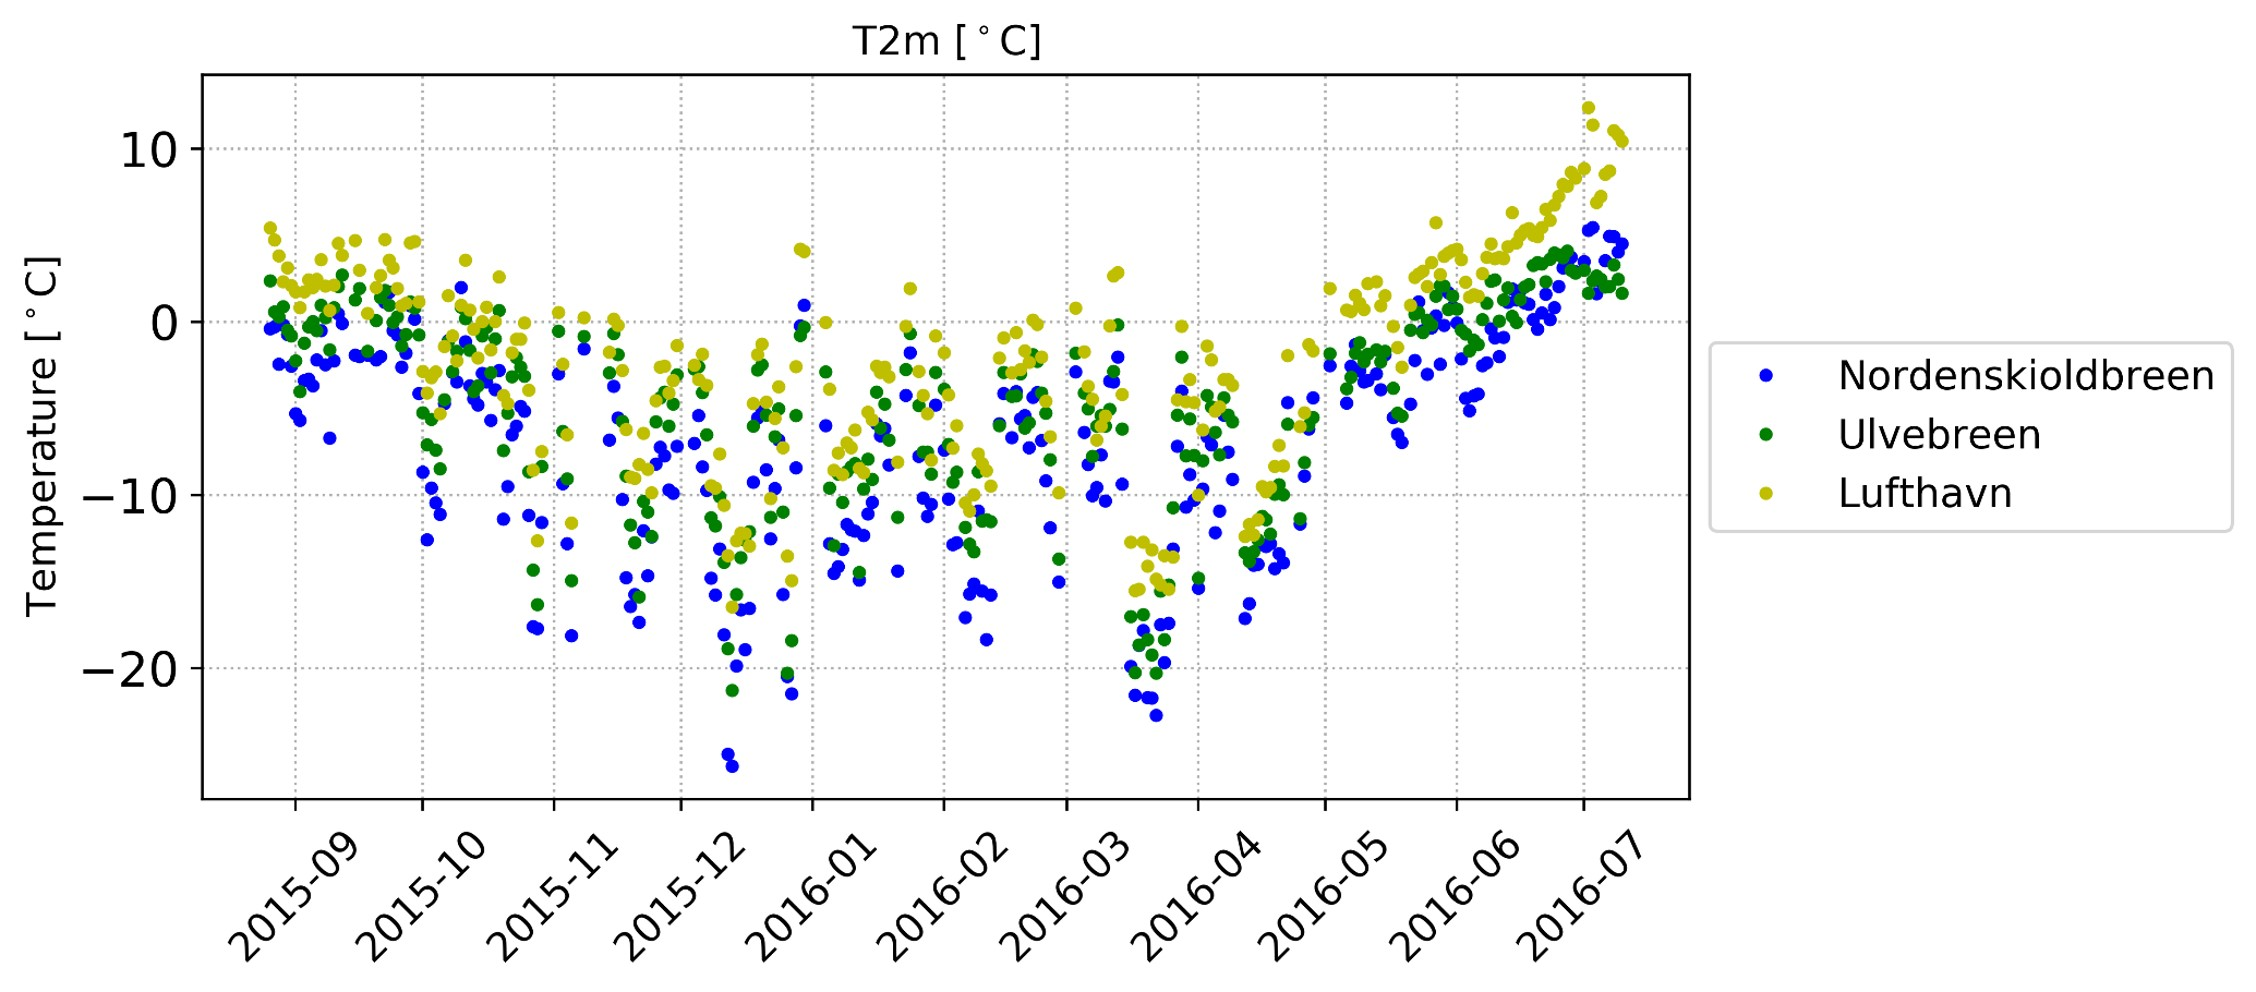
\includegraphics[scale=1, width=1\textwidth]{T2m.jpg}
    \label{fig:T2m}
    \caption{Comparison of temperature at 2 meter height for Nordenski\H{o}ldbreen, Ulvebreen and Lufthavn, where colors are corresponding to the legend.}
\end{figure}

To correct for the difference in height, for all three measurement locations the expected temperature at sea level are calculated by using the lapse rate. A lapse rate of $\SI{-6}{^{\circ}C/km}$ is used, meaning that a location at \SI{1}{km} higher should be $\SI{6}{^{\circ}C}$ colder. \todo{0.6 Source?} Calculating the expected temperature for the Nordenski\H{o}ldbreen at sea level gives:

\begin{equation}
    T_{corrected} = \SI{-7.0}{^\circ C} + \SI{6}{^\circ C/km} \cdot \SI{0.529}{km} = \SI{-3.83}{^\circ C}
    \label{eq:Tatsl}
\end{equation}

The same is done for the other two locations, giving a corrected mean temperature of $\SI{-4.04}{^\circ C}$ for the Ulvebreen and $\SI{-1.95}{^\circ C}$ for the Lufthavn. It can be noted that the mean temperatures corrected to sea level are not equal, so the difference in mean temperature is not only caused by differences in height. 

The differences in mean temperature after correcting for height are shown in table \ref{tb:avg}. To investigate if the results are significant, a t-test is done. A red cell is corresponding to a significant difference in temperature. 

\begin{table}[h]
\begin{tabular}{|l|l|l|l|l|}
\hline
\textbf{Location}          & \textbf{Height (m)} & \textbf{Nordenski\H{o}ldbreen}                      & \textbf{Ulvebreen}          & \textbf{Lufthavn}                               \\ \hline
\textbf{Nordenski\H{o}ldbreen} & 529                 & \cellcolor[HTML]{C0C0C0}{\color[HTML]{9B9B9B} } & 0.22                        & \cellcolor[HTML]{FE996B}-1.9                    \\ \hline
\textbf{Ulvebreen}         & 140                 & -0.22                                           & \cellcolor[HTML]{C0C0C0}    & \cellcolor[HTML]{FE996B}-2.0                    \\ \hline
\textbf{Lufthavn}          & 28                  & \cellcolor[HTML]{FE996B}1.9                     & \cellcolor[HTML]{FE996B}2.0 & \cellcolor[HTML]{C0C0C0}{\color[HTML]{9B9B9B} } \\ \hline
\end{tabular}
\caption{Differences (row minus column) in mean temperature (in degrees Celcius or Kelvin) between locations after correcting for height by the lapse rate. Tested by a T-test, where a red cells corresponds to a significant value.}
\label{tb:avg}
\end{table}

\todo{Hier was ik, oke}
As visible from table \ref{tb:avg}, the differences between the two glaciers are not significant, while the difference between the Lufthavn and a glacier is significant. This is probably due to the fact that the Lufthavn is not a glacier and has a lower average albedo. Thereby, in summer, the average temperatures of glaciers usually are not rising above 0 degrees Celsius, because the energy from the heat is converted into melt energy.\\

Since temperatures at two meter are interpolated from other variables for the Nordenski\H{o}ldbreen and Ulvebreen, the surface temperature of both glaciers Nordenski\H{o}ldbreen and Ulvebreen are compared with each other, visible in figure 
\ref{fig:Tsurf}. Again, this is only done for the period with overlapping data. Looking through the different values at the axis, the Nordenski\H{o}ldbreen looks colder. To correct for this, again the lapse rate is used of 2,3 degrees which is added to the data, corresponding to the black line in figure \ref{fig:Tsurf}. For example, when a temperature of -10 degrees Celcius is reached at the Ulvebreen, it has to be -12,3 degrees at Nordenski\H{o}ldbreen when corrected for height. With this lapse rate, it is 0.15 degrees Celcius warmer at the Ulvebreen than expected. Again, a T-test is done for the difference in surface temperatures for both glaciers. With a p-value of 0.7, the Ulvebreen is not significant warmer than the Nordenski\H{o}ldbreen.

\begin{figure}[h]
\centering{}
    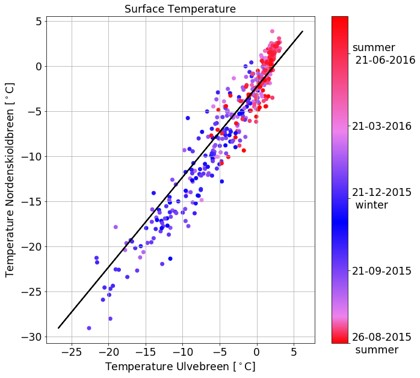
\includegraphics[scale=0.5, width=0.5\textwidth]{Tsurf.jpg}
    \label{fig:Tsurf}
    \caption{Comparison of surface temperature of Ulvebreen, visible at the x-axis and the Nordenski\H{o}ldbreen, visible at the y-axis. In colors, the dates are visible from summer 2015 in red below, via winter 2015 in blue, to summer 2016 above, again in red. For explanation of the black line, see text.}
\end{figure}

To conclude, taking into account the lapse rate, the temperatures overlap really well. So, the temperature differences between the locations of the measurement are related to the height of the measurements.

However, also visible in figure \ref{fig:Tsurf} are the temperatures which are slightly above 0 degrees for both glaciers. This is not expected, because at a value of 0 degrees, the ice will melt and the energy will be converted. To investigate this furthermore, the incoming shortwave radiation is compared with the wind speed and hut temperature for the Nordenski\H{o}ldbreen. For this, all years of data of the Nordenski\H{o}ldbreen is used between 21 June and 21 September. This is plotted in figure \ref{fig:Thut}. If the sensor is influenced by the wind speed, we expected a higher temperature of the surface at a lower wind speed and a high incoming surface radiation. This is recognizable to the dark red dots at the left upper corner. With this, we can conclude that the sensors of surface temperature of both glaciers do probably have a small uncertainty.

\begin{figure}[h]
\centering{}
    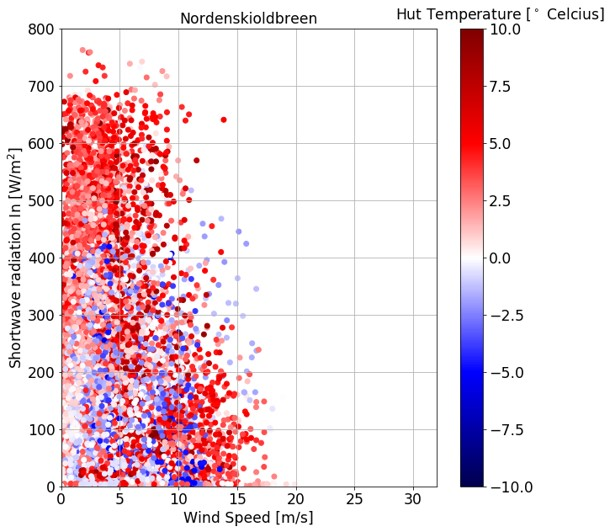
\includegraphics[scale=0.5, width=0.5\textwidth]{Thut-Sin.jpg}
    \label{fig:Thut}
    \caption{Comparison of the wind speed at the x-axis, the incoming shortwave radiation at the y-axis and the surface temperature corresponding to the colorbar at Nordenski\H{o}ldbreen for all available years between 21 June and 21 September (summer) }
\end{figure}

\section{Prevailing winds}\label{sec:katw}
Next to the temperatures of the glaciers, differences in wind direction and wind speed are investigated. This is done for both glaciers apart, to take into account all data points of each glacier. Results are visible in figure \ref{fig:PR}.

\begin{figure}[h]
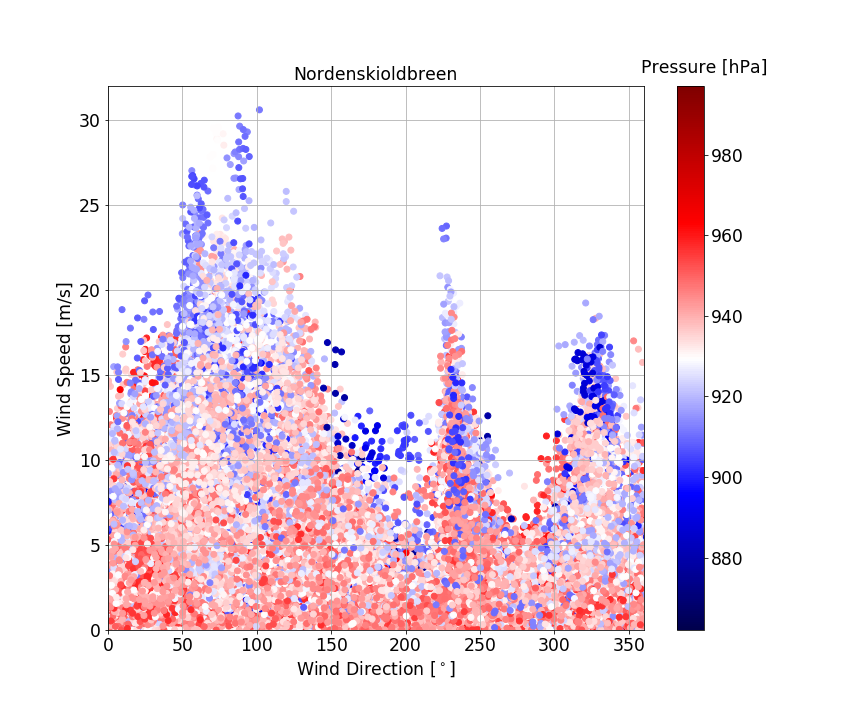
\includegraphics[scale=1, width=0.5\textwidth]{WD-WS-PR-Nordenskioldbreen.png}
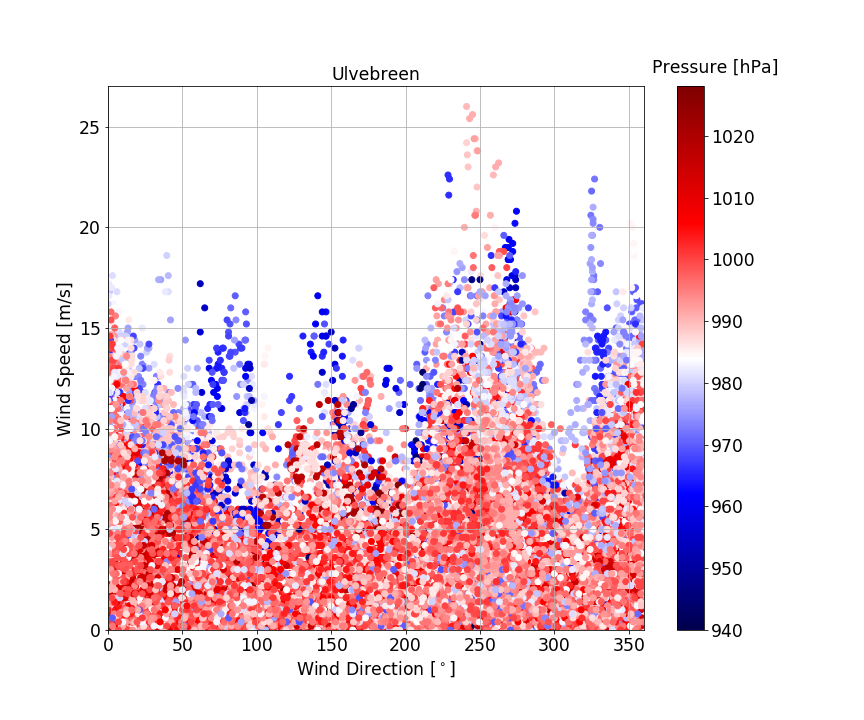
\includegraphics[scale=1, width=0.5\textwidth]{WD-WS-PR-Ulvebreen.png}
\caption{Comparison of the wind direction at x-axis, wind speed at y-axis and the corresponding pressure, related to the colorbar. Left: Nordenski\H{o}ldbreen and right: Ulvebreen}
\label{fig:PR}
\end{figure}

Within these plots, clearly visible are the lower values of pressures at higher wind speeds and vice versa. These are caused by the synoptic atmospheric low pressure system. Some wind directions can reach higher wind speeds, for example at the Nordenski\H{o}ldbreen at around 60 degrees and at the Ulvebreen at 250 degrees. To investigate this furtermore, the differences in temperatures between two meter and surface are plotted instead of the related pressure, which is visible for the Nordenski\H{o}ldbreen in figure \ref{fig:PRnorde} and for the Ulvebreen in figure \ref{fig:PRulve}. Remarkable wind directions and wind speeds refer to coloured arrows. In red, the arrow corresponds to the katabatic wind, where wind is blowing down glacier corresponding to higher wind speeds and a warmer temperature at 2 meter instead of the surface temperature. This is because of the horizontal pressure gradient. At the right side in those figures, the map is plotted with the location of the weather station and the corresponding coloured arrows. 

\begin{figure}[h]
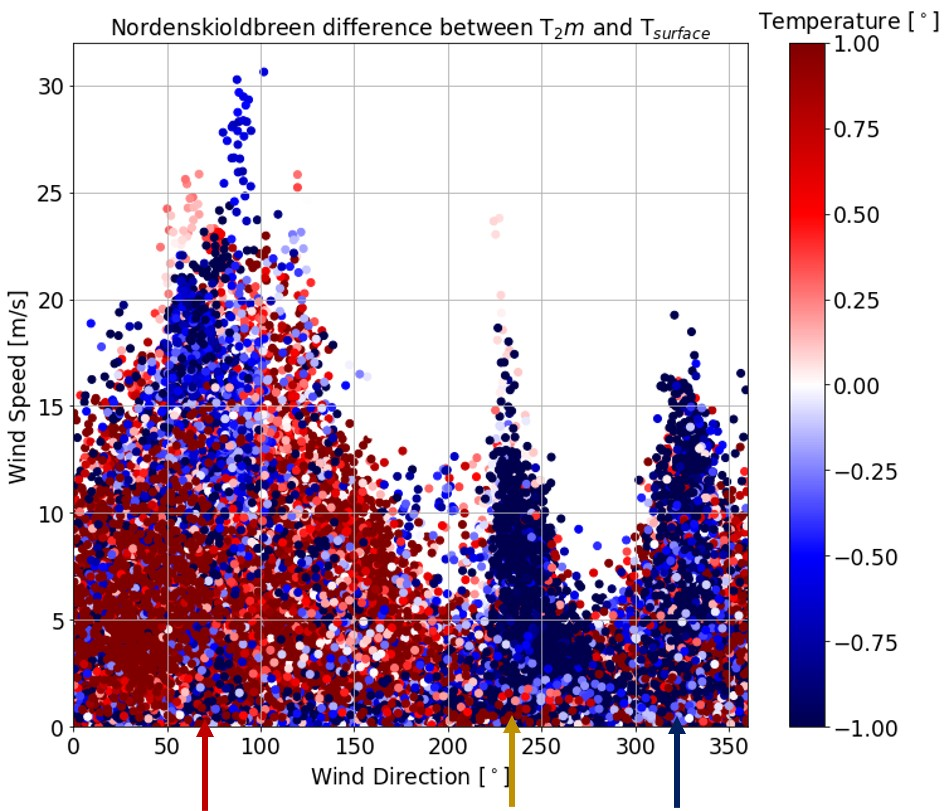
\includegraphics[scale=1, width=0.55\textwidth]{ulve-WS-WD.jpg}
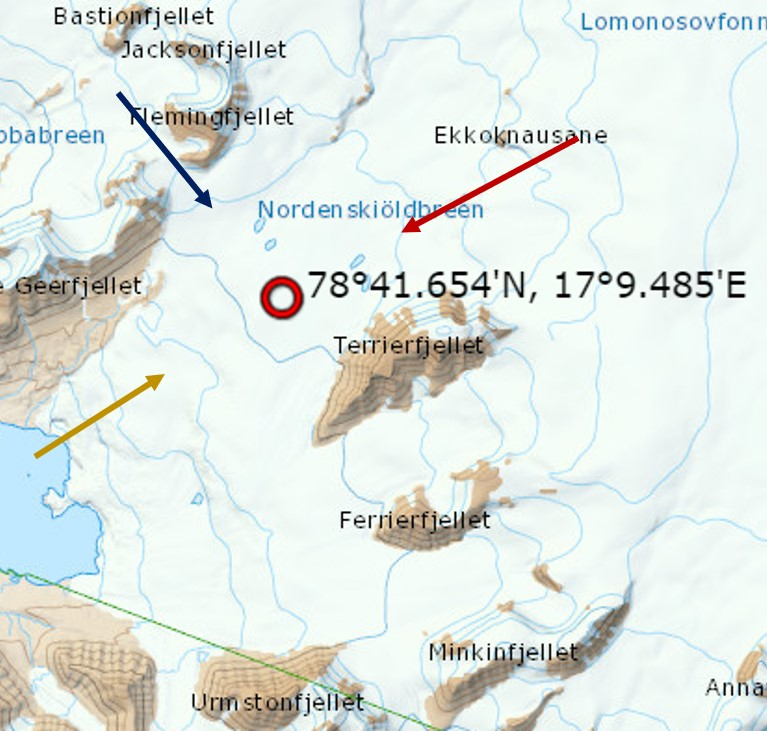
\includegraphics[scale=1, width=0.45\textwidth]{norde-WS-WD-rose-2.jpg}
\caption{Left: Comparison for the Nordenski\H{o}ldbreen of the wind direction at x-axis, wind speed at y-axis and the corresponding pressure, related to the color bar. Right: Maps with wind directions, related to the colored arrows. In red temperature at two meter is higher than the surface temperature, conversely in blue.}
\label{fig:PRnorde}
\end{figure}

As can be seen in figure \ref{fig:PRnorde}, the wind directions overlap really well with the expected wind directions related to higher wind speeds; wind is coming down glacier at 60 degrees and from the bay up glacier at 240 degrees. This is probably caused by wind blowing through the fjord and tunneling in the bay. A third peak is visible at 320 degrees where wind is coming from the saddle. Thereby between roughly 0 and 50 degrees, a bigger spectrum of relatively high wind speeds are visible. This is presumably because of the different possible corners.

\begin{figure}[h]
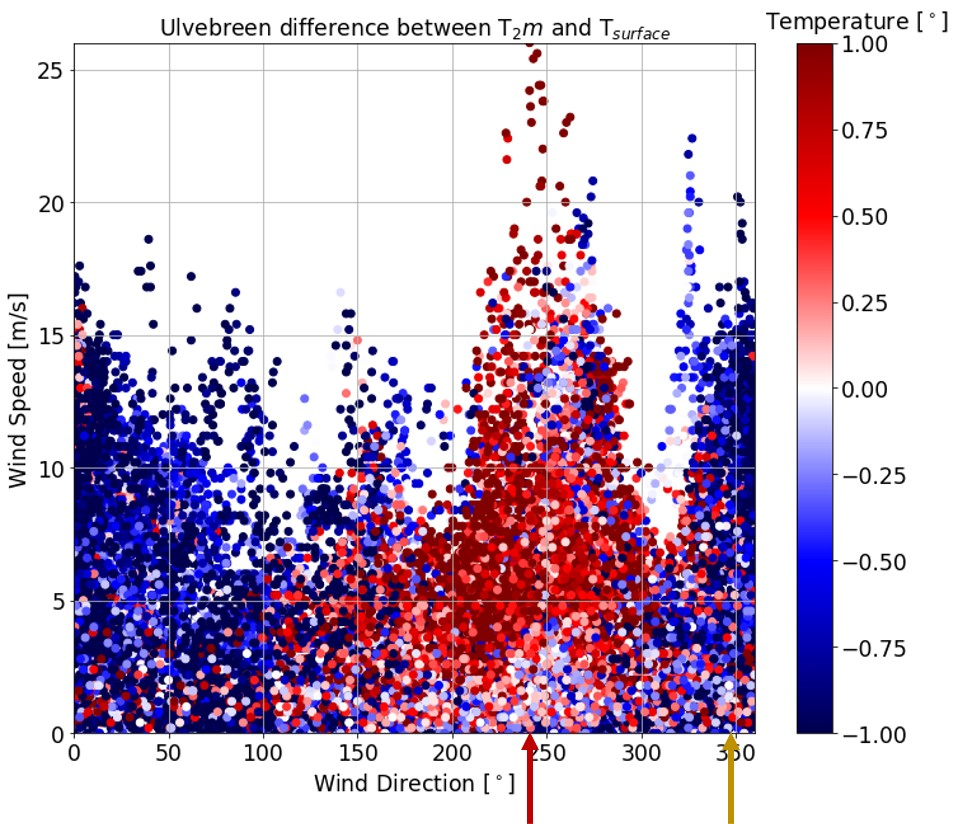
\includegraphics[scale=1, width=0.6\textwidth]{norde-WS-WD.jpg}
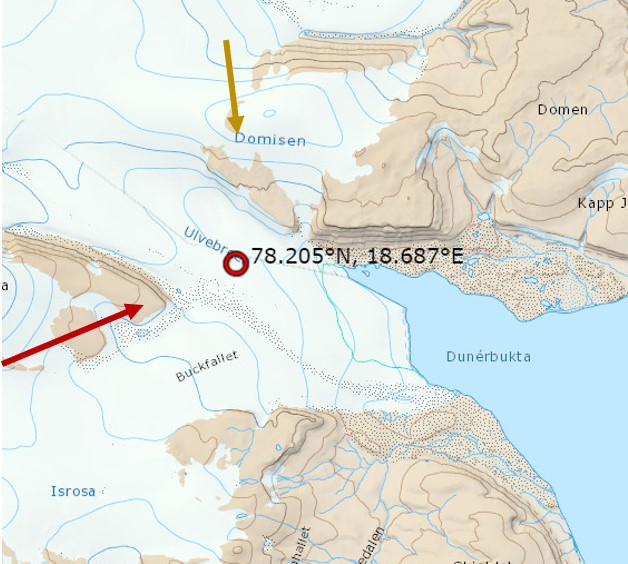
\includegraphics[scale=1, width=0.40\textwidth]{ulve-WS-WD-rose-1.jpg}
\caption{Left: Comparison for the Ulvebreen of the wind direction at x-axis, wind speed at y-axis and the corresponding pressure, related to the color bar. Right: Maps with wind directions, related to the colored arrows. In red temperature at two meter is higher than the surface temperature, conversely in blue.}
\label{fig:PRulve}
\end{figure}

However, as visible in figure \ref{fig:PRulve}, at the Ulvebreen, wind directions are not overlapping with expectations. For example, higher wind speed at a wind direction of 240 degrees is corresponding to a wind uphill. The results are more overlapping with expectations when turning both arrows for about 15 degrees to the left. In this case, both wind arrows are corresponding to down-glacier winds. This is probably caused by a veering part of the construction of the instrument.

\section{Snow and albedo}\label{sec:rad}
In this section, the relation between snow height and albedo of the Nordenski\H{o}ldbreen and the Ulvebreen is furthermore investigated. First, a plot is made of the albedo and uncorrected snow height for the average values at the overlapping dates of the Nordenski\H{o}ldbreen and the Ulvebreen, as shown in figure \ref{fig:S1}. In this case, the snow surface height is called uncorrected, because values are related to the distance from the sensor above the surface to the snow surface. For example, low values means a small distance, which means a lot of snow, corresponding to a high snow surface.

\begin{figure}[h]
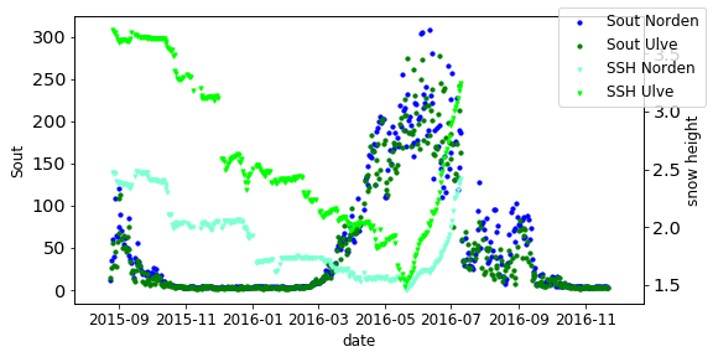
\includegraphics[scale=1, width=1\textwidth]{Picture1.jpg}
\caption{Snow surface height ("Uncorrected", see text) corresponding to the triangles and albedo corresponding to the dots, as visible in the legend for both glaciers, Nordenski\H{o}ldbreen and Ulvebreen at the overlapping dates.}
\label{fig:S1}
\end{figure}

Visible are snow showers prevailing in winter, where each situation of snow shower has its own impact at the glacier. When the days are "longer" with more incoming Solar radiation, the values of albedo are decreasing. Between May and June of 2016, at the beginning of the summer, when the uncorrected snow height is increasing, the melting starts. Correlated to this, the albedo's are decreasing again, because snow does not reflect as much radiation as ice. Also visible are relatively higher values of albedo of the Ulvebreen before melting starts, because the ice of the Nordenski\H{o}ldbreen is more dirty. However, the overlap in days are not long enough to cover the full cycle. To investigate the whole cycle, the data is examined for each glacier apart. 

The albedo and snow height are compared for the Ulvebreen, visible in figure \ref{fig:S2}. In this case, the snow height is "corrected". This means the smallest value of the uncorrected snow height is set to zero and from there on, the snow height is calculated. In this plot, the differences between winter and summer are more obvious. In the beginning, when snow showers occur, the albedo increase rapidly. Between the black dotted parts, after May of 2016, the melt starts, where fresh snow covers the old snow and the albedo starts to decrease. If the melt ends and the old snow becomes ice, the albedo jumps to much lower values. After this, a few snow fall events with slightly higher the snow height, but the albedo increases rapidly. This cycle is roughly repeating itself at the Ulvebreen between 2015 and 2018. 

\begin{figure}[h]
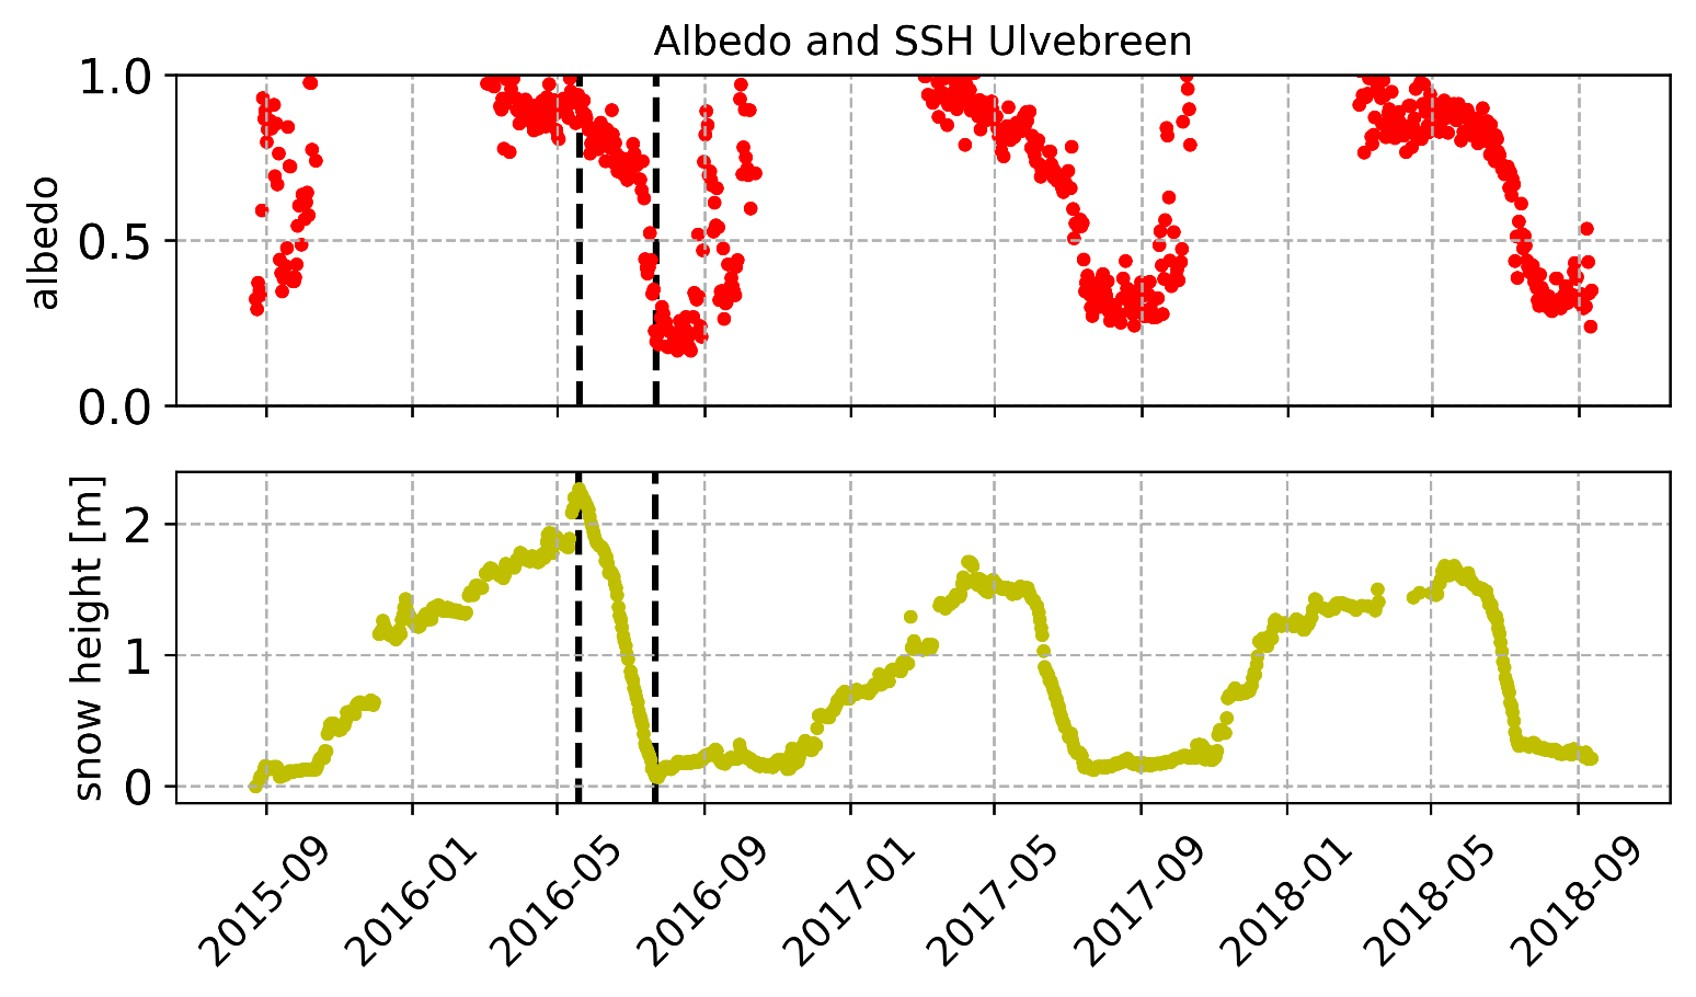
\includegraphics[scale=1, width=1\textwidth]{Picture2.jpg}
\caption{Above: Snow surface ("corrected", see text) height and below: albedo calculated for each data point of the Ulvebreen.}
\label{fig:S2}
\end{figure}

Also, the albedo and snow height are compared for the Nordenski\H{o}ldbreen, visible in figure \ref{fig:S3}. Again in this case, the snow height is "corrected". However, the snow height sensor here works different compared to the Ulvebreen. The snow height sensor is drilled in the ice, so differences in height are because of differences in both snow and ice height. To compare the snow height and albedo, a lot of values are inclued. Due to the gaps in one of the necessary values, measurements at the Nordenski\H{o}ldbreen are not contineous and thereby, no stable summer period is considered, so the correlation between the albedo and snow height is less visible in the plots of figure \ref{fig:S3}.  \todo{black dotted parts?}

\begin{figure}[h]
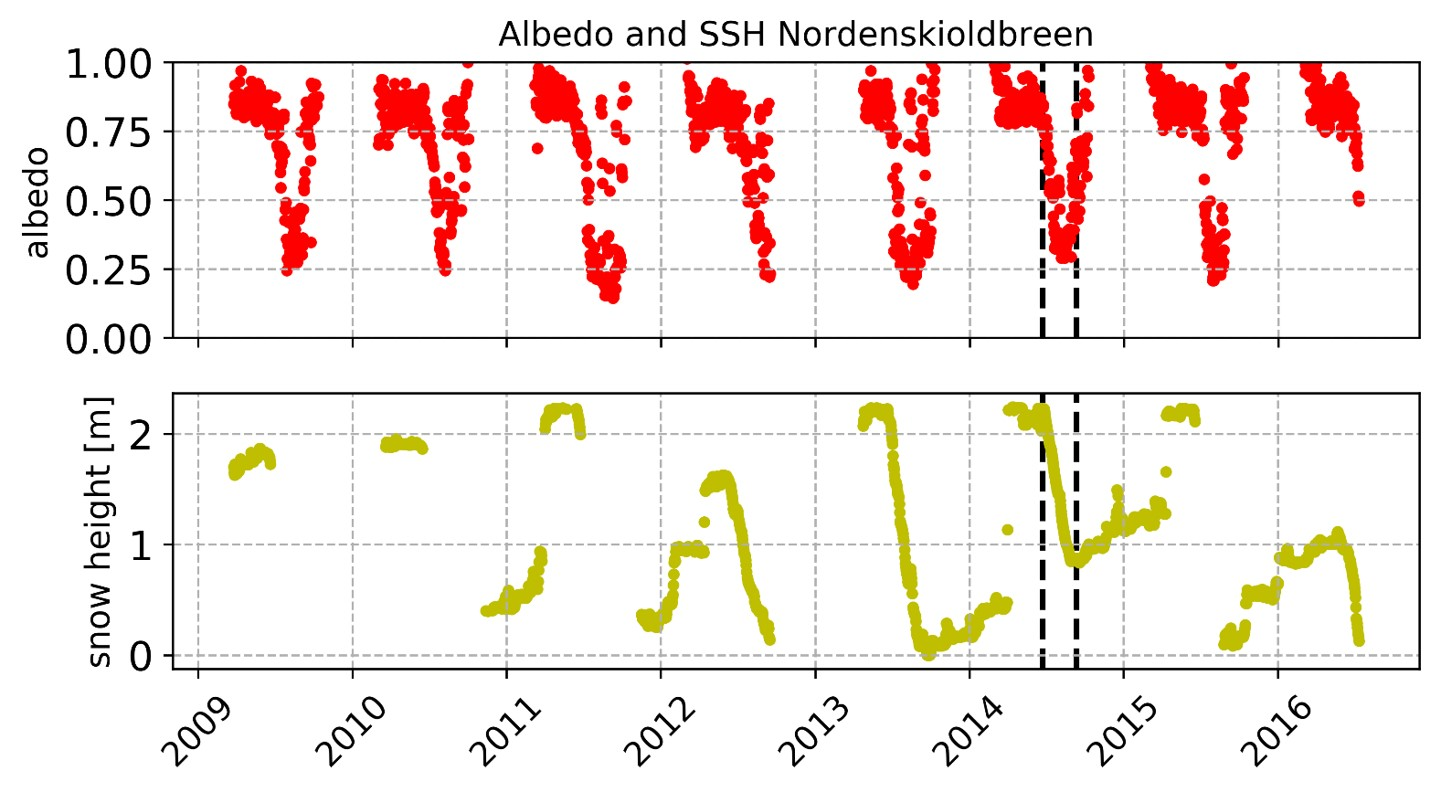
\includegraphics[scale=1, width=1\textwidth]{Picture3.jpg}
\caption{Above: Snow surface ("corrected", see text) height and below: albedo calculated for each data point of the Nordenski\H{o}ldbreen.}
\label{fig:S3}
\end{figure}

\chapter{Discussion}\label{sec:discussion}

\section{Temperature}\label{sec:Tdisc}
Temperature
On the western side, you will have higher temperatures compared to the E side because of the Gulf Stream. 
N-S = latitude logica.

However, the differences between the are raised because the nordenskioldbreen (blue) is located more northward and thereby in the same temperature band as the ulvebreen (green), which overlaps with our results.

Lufthavn more westward, so warmer. 


\begin{figure}[h]
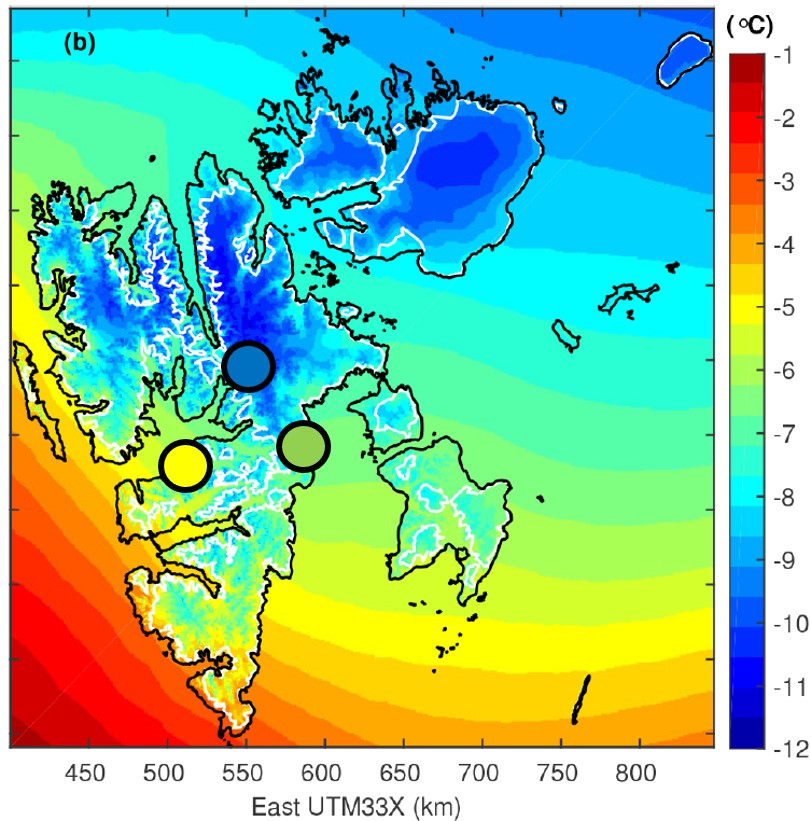
\includegraphics[scale=1, width=0.5 \textwidth]{ostby.jpg}
\cite{osby}
\caption{Annual mean air temperature at 2 meter averaged over 1979 to 2014 from ERA-Interim}
\label{fig:trossby}
\end{figure}
\todo{including dots}

\section{Prevailing winds}\label{sec:pw}
\todo{what to write?}

\section{Snow and albedo}\label{sec:sa}
\todo{what to write?}



\chapter{Conclusion}\label{sec:conclusion}

\textcolor{red}{
Main differences because of height (Temperature)
No big differences in local climate (Significant)
Measurement uncertainties (Temperature, Snow height, Albedo, Wind direction)
Temperatures are highly dependend on location of latitude and longitue and height\\
direction glacier related to Wind direction and katabatic wind\\
differences in albedo related to different Sin in time and amount, dirty snow/ice}

%"Vijf jaar na de succesvolle eerste SEES.NL expeditie, willen we graag weer terug om de veranderingen vast te leggen. Het concept is net als in 2015. Allerlei wetenschappers aangevuld met toeristen. We hebben hulp nodig om dit mogelijk te maken. Geef je vrijblijvend op als wetenschapper, toerist of sponsor. Dan nemen we snel contact met je op."

\medskip

\begin{thebibliography}{9}
\addcontentsline{toc}{chapter}{Bibliography}
\bibitem{sval}
Website: The University Centre in Svalbard, UNIS (01-2018), 
\textit{The Early Exploration of the Arctic and the Discovery of
Svalbard},
Retrieved at 30-10-2018, from:\\
\texttt{\small{https://www.unis.no/wp-content/uploads/2018/01/SH201\_Summary02\_2018.pdf}}

\bibitem{sees}
Website: Netherlands Scientific Expedition Edgeøya Spitsbergen, SEES, (2015), \\ Retrieved at 30-10-2018, from:
\texttt{\small{http://www.sees.nl/}}\\

\bibitem{abl}
Article: Hulth, J. (2010). 
\textit{Using a draw-wire sensor to continuously monitor glacier melt.} Journal of Glaciology, 56(199), 922-924. 
\texttt{doi:10.3189/002214310794457290}

\bibitem{uuproj}
Website: Institute for Marine and Atmospheric Research (IMAU)
\textit{Ice and Climate: Automatic Weather Stations on glaciers}
Retrieved at 30-10-2018, from:
\texttt{https://www.projects.science.uu.nl/iceclimate/aws/files\_oper/}

\bibitem{1}
Website: Norwegian Meteorological Institute Svalbard climate data
\textit{Weather statistics for Longyearbyen (Svalbard)},
Retrieved at 30-10-2018, from:
\texttt{https://www.yr.no/place/Norway/Svalbard/Longyearbyen/statistics.html}


\bibitem{2}
Article: Storrie, Luke, Lydersen, Christian, Andersen, Magnus, B.Wynn, Russell and Kovacs, Kit. (2018). 
\textit{Determining the species assemblage and habitat use of cetaceans in the Svalbard Archipelago, based on observations from 2002 to 2014.} Polar Research. 37. 10.1080/17518369.2018.1463065. 

\bibitem{sharkii}
Website: eKlima \textit{the climate database of the Norwegian Meteorological Institute}, Retrieved at 30-10-2018, from:
\texttt{http://sharki.oslo.dnmi.no/}

\bibitem{osby}
Article: Østby, T. I., Schuler, T. V., Hagen, J. O., Hock, R., Kohler, J., and Reijmer, C. H.: \texttt{Diagnosing the decline in climatic mass balance of glaciers in Svalbard over 1957–2014}, 
The Cryosphere, 11, 191-215 \texttt{https://doi.org/10.5194/tc-11-191-2017}, 2017.

\end{thebibliography}

%\chapter*{Appendices}
%\addcontentsline{toc}{chapter}{Appendices}

%\section*{A. name}\label{Ap:A}
%\setcounter{figure}{0}
%\renewcommand{\thefigure}{A.\arabic{figure}}
%\addcontentsline{toc}{section}{A. name}



\end{document}
